\documentclass[a4paper,10pt]{article}



\usepackage{listings}
\usepackage[english]{babel}
\usepackage{graphicx}
\usepackage[colorlinks, linkcolor=black, citecolor=black, urlcolor=black]{hyperref}
\usepackage{geometry}
\geometry{tmargin=3cm, bmargin=2.2cm, lmargin=2.2cm, rmargin=2cm}
\usepackage{todonotes} %Used for the figure placeholders
\usepackage{ifthen}


%=== TITLE & AUTHORS ====================================================================
\begin{document}

\title{Execution models}
\author{Maria I. Artigas}

% The paper headers
% \markboth{IEEE TRANSACTIONS ON MICROWAVE THEORY AND TECHNIQUES, VOL.~60, NO.~12, DECEMBER~2012
% }{Roberg \MakeLowercase{\textit{et al.}}: High-Efficiency Diode and Transistor Rectifiers}


% ====================================================================
\maketitle



% === ABSTRACT ====================================================================
% =================================================================================
\begin{abstract}
%\boldmath

\end{abstract}


% === KEYWORDS ====================================================================
% =================================================================================
\begin{IEEEkeywords}
Higher order reasoning, knowledge graphs, petri nets
\end{IEEEkeywords}



% ====================================================================
% ====================================================================
% ====================================================================


% === I. INTRODUCTION =============================================================
% =================================================================================
\section{Introduction}

This document aims to explain methods for coordination of resources in the context of Assembly Execution System in AssemblyRecon and an assembly case in PROUD. The structures presented here aim to help representing and coordinating the execution of multi robot tasks,  with time extended assignments and multi task robots according to the classification in \cite{korsah2013comprehensive}. 

Small introduction on how the purpose of this report is to make a link between declarative constraints among tasks and resources, with the coordinated execution of them given the resource-task allocation.

\section{Task dependency relations }


A minimal set of relations is presented in this section for structuring partial task specifications.  This relations aim to provide needed dependencies on what has to be done, using which capabilities.
As previously mentioned, the declarative structure presented aim to provide a base to declare multi robot tasks, with extended assignments and multi task robots. 
For this purpose, the set of relations for the task specification should also allow linking task specification with the resource capabilities required for execution.
The set of relations can be divided in two major sets: task interdependencies, and dependencies between task and capabilities of resources. % RETHINK IF MENTIONING RESOURCES OR CAPABILITIES, AS YOU ARE DOING THE SWITCH WITHOUT PREVIOUSLY MENTIONING THE LINK

The data structure used to store task specification in this work is linked data. This is due three main reasons:
\begin{itemize}
    \item Flexibility to link different types of data, independently of content or granularity. (This allows to perform similar methods of decision making on different levels of granularity of the data).
    \item Flexibility of internal structures. As it is based on triples, internal structures do not constraint the linking of data.
    \item Accessible entry to the data through semantic queries.
\end{itemize}
%ADD EXAMPLE OF GRAPH
\subsection{Task interdependencies}
% MAKE THE RIGHT CITATION

Cyber-physical systems tasks % are defined and constraint by dependencies among tasks and other situation information
% In cyber phisical tasks are continuous on time, which is why their performance has as key character its duration
% for this reason, when having contraints between tasks, the duration characterization has to be taken into account.
The temporal constraints it contains can be described from interval theory graph representations \cite{1}.
From this work the temporal interval relations to be inherited are (see figure \ref{fig:allens_framework}): \\
$\{ before ,meets ,overlaps ,starts ,during ,finishes ,equal \}$.
\\
\begin{figure}[h]
    \centering
    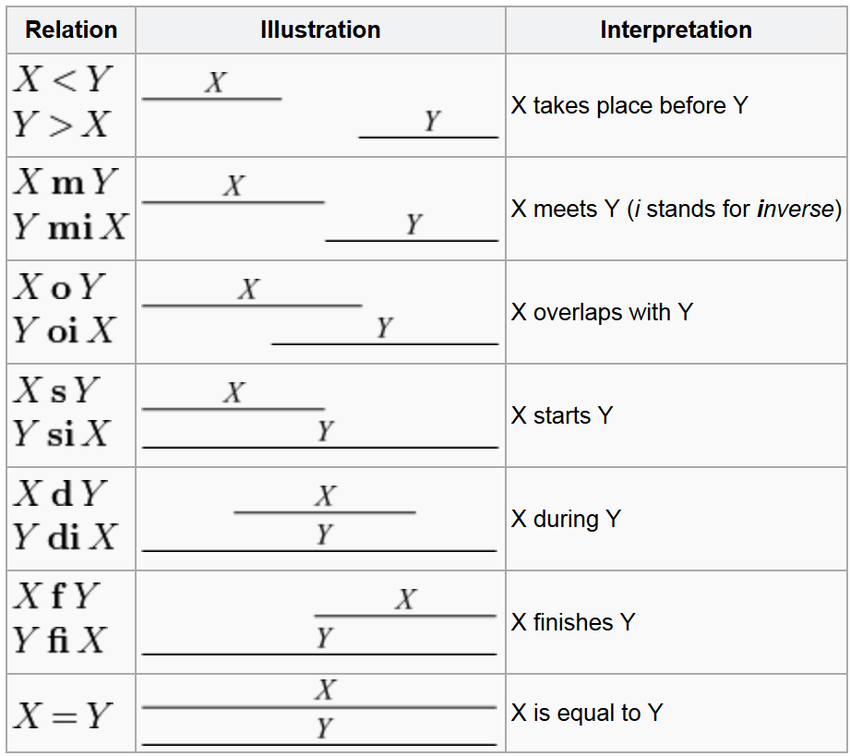
\includegraphics[width=0.5\textwidth]{allens_framework.png}
    \caption{Allen's framework relations}
    \label{fig:allens_framework}
\end{figure}



%ADD THAT TO INTRODUCE TIME DEPENDENCY CONTRAINTS YOU NEED TO DEFINE WHICH PART OF THE RELATION HOLDS THAT DEPENDENCY
The task can be expressed as a set of subtasks which are interrelated with the previous relations in a directed manner. According to the definition in \cite{1}, we can appreciate that the definition of direction of the relation indicates the precedence between the tasks, aside from the equal relation. The equal relation can be defined as bidirectional there is no precedence among the tasks.
\\

To this work, the concept of necessity has to be added. Who needs this relation to hold? 
For example, task a and b can be equal. When perform task a, task a needs task b to be performed at the same time (equal relationship). However, task b might not need task a to be performed simultaneously. For example, to move a rotor (task a) we need the gripper to be actively closed (task b), but the gripper can be actively closed also in other situations not including the performance of moving the rotor. 
\\

When taking the subgraph from the task composed by the nodes which are related by \textb{before} relation, this subgraph is a directed acyclic graph. The cause of this is the requirement on the lack of loops in the execution. 
The composed graph (with the other relations included) allows the expression of different paths to execute the same task, which composes a more robust execution, given the choice of different executions for the same task.

\subsection{Dependencies between task and capabilities of resources}

The execution of these tasks can be realized by a set of capabilities of the resources. 
The declaration of capabilities in this work is done as an tree structure with the relations 

From the point of view of execution of tasks, the minimum relations needed for the characterization of the resources (active) % CHECK IF IT ALSO HOLDS FOR PASSIVE RESOURCES
are the mereological (check) description of the resources and the topological description of the resources available. This data forms the base information for checking the feasibility of tasks and their following allocation.

The mereological description 

% Introduce the tree structure over capabilities
% Introduce the relation with the particular resources
% Introduce the relation to the category of resources


The link between the task and the resources is defined by the capabilities which can provide the task. In the paradigm of linked data, this is represented as the relation %{FILL ME IN}
% You can describe that the good thing of this description is good as you can do it at any level of granularity of capabilities or part in the resource tree, but I find it redundant with the introduction on link data, though you can mention it on the examples part


\subsection{PROUD: Skill Execution Graph}

For demonstration of the previous approach, an illustration case is the assembly of an snapfit. In this case, the resource available is a industrial arm manipulator with a gripper as end effector.



\subsection{AssemblyRecon: Product Execution Graph}

AML /ISA 95 and translation to these concepts

Task + resource = skill for the resource

Assembly graph ???

The transition tasks in the model are described as:

\begin{figure}
\begin{lstlisting}

  {
    "@id": "http://kuleuven.com/grip_rotor",
    "http://kuleuven.com/needs_precondition": [
      {
        "@id": "http://kuleuven.com/move_to_rotor"
      },
      {
        "@id": "http://kuleuven.com/rotor_visual_check"
      }
    ],
    "http://kuleuven.com/needs_capabilities": [
      {
        "@id": "http://kuleuven.com/move_cartesian"
      },
      {
        "@id": "http://kuleuven.com/visual_check"
      },
      {
        "@id": "http://kuleuven.com/grip"
      }
    ]
  }
\end{lstlisting}
\end{figure}

Task interdependencies example:

Bill of materials:


Bill of resources:

Capabilities of resources: 

CONTINUE MODEL WITH PAGE 219 -> DUAL LEVEL TASK SPECIFICATION: GUARDED ORDER EXECUTION 


\section{Task dependency model to task execution model}

Given the task specification as the structure presented in the previous section, the next step towards execution, is the connection to required coordination models.

Every task (which was represented as a subgraph or node in the previous section), should be composed with the resource capabilities information in order to compose the coordination required for its execution. This composition is developed with 2 types of models in this work: finite state machines and petri nets.

\subsection{Task dependency model to task execution model: Petri net coordination}


Petri nets are chosen as coordination method. For it, the main aim is to translate the declared dependencies between task-task and task-resource to the petri nets, so the petri net contains the required information for synchronized work of shared resources.\\

%ADD SMALL DESCRIPTION OF PETRI NETS 

For the connection of petri net structures with task dependencies described at section \ref{section_1}, semantic conventions have to be added to the petri nets.
\begin{figure}[h]
    \centering
    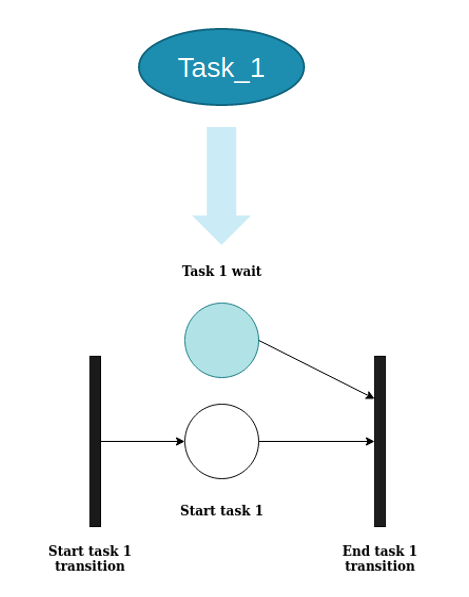
\includegraphics[width=0.5\textwidth]{task1_petri.png}
    \caption{Task representation in petri net}
    \label{fig:task1_petri}
\end{figure}

CONVERSION BETWEEN NODE AND PLACE 
CONVENTIONS TO TRANSLATE FROM RELATIONS TO STRUCTURES IN PETRI NETS
CONVENTIONS REGARDING RESOURCE NODES AND RESOURCE PLACES


The placement of a token can have different semantic meaning given its simplicity.

For this purpose, the previous temporal interval constraints as $\{ before ,meets ,overlaps ,starts ,during ,finishes ,equal \}$
are the relation primitives for the declaring temporal constraints between tasks.

Regarding execution of the tasks

This is because in the petri net, the granularity at the task/skill level is not relevant, given the flags and tokens are filled in accordingly.

In this context, the granularity of detail 


One petri net per task (one mediator per petri net)





One communication channel per resource (one communication mediator per resource)

\subsection{Task dependency to task execution models: LFSM reactivity}



\section{Stable states in petri nets and fsms}

\section{Progress metrics extracted from petri nets and fsms}

Flag copy per resource 
Node in the fsm


\section{Preemption/backtracking at the level of petri nets and fsms}

High order flags to be added to the petri nets = timeouts, active ...(lcsm states), highwater, lowwater 
Page on preemption reasoning from what I wrote in the notebook

\section{Skill table between petri nets for task/resource/skill correlations}

\section{Communication protocol (optional)}
Flags and communication information 

Metadata regarding association between communication protocol and petri net generation -> 


\subsection{AssemblyRecon: task-resource/skill table}

Also talk about where to keep the state of the tool in the resource holon and then doing the preemption accordingly


\section{Delay impact regarding preemption/backtracking/contingency plans/rush orders}
\textcolor{cyan}{Here -> need to talk about critical resources, how you can predict the cascading and so on and so forth}

\section{Conclusion}

\section{Notes}

Make references to petri net plans (from https://sites.google.com/a/dis.uniroma1.it/petri-net-plans/publications?authuser=0) maybe in the introduction add the added value of this work over that. (Also as added value -> petri net mediator and flags -> make connections automatically with the agents instead of the agents having to keep up with the petri net)


\section*{Acknowledgment}

\bibliographystyle{abbrv}
\bibliography{bibliography.bib}
\end{document}



